%%
% La siguiente plantilla esta basada en el siguiente enlace:
% http://academic.reed.edu/physics/courses/Physics332.s08/reports.html
% La plantilla original puede descargarse de ese sitio
% Se dejo parte del texto original en inglés para ilustar el uso de la plantilla
% Se hicieron algunas modificaciones para ajustar el idioma y otros detalles para 
% completar un reporte técnico breve pero muy puntual
% Modificación Inicial: Marco Aurelio Nuno Maganda - 11/SEP/2014
% 
% Enlace a la documentación del tipo de documento base (revtex4)
% http://mirror.hmc.edu/ctan/macros/latex/contrib/revtex/doc/latex/revtex/source/revtex4-1.pdf
%
% En algunas distribuciones es necesario instalar el paquete texlive-publishers
%
%\documentclass[letterpaper,aps,twocolumn,pre,nofootinbib]{revtex4}
%\documentclass[twocolumn]{article}
\documentclass[conference]{IEEEtran}

\usepackage[spanish]{babel}
\usepackage{amsmath,amssymb,amsfonts,amsthm}
\usepackage{graphicx}
%\usepackage{bbm}
\usepackage[utf8]{inputenc} % Caracteres en Español (Acentos, ñs)
\usepackage{url} % ACENTOS
\usepackage{hyperref} % Referencias
\usepackage{subfig}
\usepackage{lipsum}
\usepackage{balance}


\usepackage{graphicx} % Required for including images
\usepackage[font=small,labelfont=bf]{caption} % Required for specifying captions to tables and figures


\usepackage{tikz}
\usetikzlibrary{automata, positioning, arrows}

%%%%%%%%%%%%%%%%%%%%%%%%%%%%%%%%%%%%%%%%%%%%%
% PARCHE PARA ELIMINAR LA FECHA DEL DOCUMENTO
% 
\usepackage{etoolbox}
\makeatletter
% \frontmatter@RRAP@format is responsible for the parentheses
\patchcmd{\frontmatter@RRAP@format}{(}{}{}{}
\patchcmd{\frontmatter@RRAP@format}{)}{}{}{}
%\renewcommand\Dated@name{}
\makeatother	
% FIN DEL PARCHE
% 
%%%%%%%%%%%%%%%%%%%%%%%%%%%%%%%%%%%%%%%%%%%%%

%%%%%%%%%%%%%%%%%%%%%%%%%%%%%%%%%%%%%%%%%%%%%
% PARCHE PARA PERMIRIR UTILIZAR BIBLATEX EN ESTA PANTLLA
%\PassOptionsToPackage{square,numbers}{natbib}
%\RequirePackage{natbib}  
%%%%%%%%%%%%%%%%%%%%%%%%%%%%%%%%%%%%%%%%%%%%%

\usepackage[backend=bibtex,sorting=none]{biblatex}
% Estas lineas permiten romper los hipervinculos muy largos !!!!
\setcounter{biburllcpenalty}{7000}
\setcounter{biburlucpenalty}{8000}
\addbibresource{references.bib}

% Actualiza en automático la fecha de las citas de internet a la fecha de la compilación del documento
\usepackage{datetime}
\newdateformat{specialdate}{\twodigit{\THEDAY}-\twodigit{\THEMONTH}-\THEYEAR}
\date{\specialdate\today}

% la sentencia \burl en las citas... 
\usepackage[hyphenbreaks]{breakurl}

\renewcommand\spanishtablename{Tabla}
\renewcommand\spanishfigurename{Figura}



\begin{document}

\newcommand{\breite}{0.9} %  for twocolumn
\newcommand{\RelacionFiguradoscolumnas}{0.9}
\newcommand{\RelacionFiguradoscolumnasPuntoCinco}{0.45}



\title{Reporte de Proyecto Grupal 1 \\Graphs}

\author{\IEEEauthorblockN{Moreno Ledesma Ximena Abigail\IEEEauthorrefmark{1},
Palmero Torres Javier Martín\IEEEauthorrefmark{1},\\
Ruiz Marquez Adrián Alejandro\IEEEauthorrefmark{1} y 
Torres Colorado Juan Daniel \IEEEauthorrefmark{1}}
\IEEEauthorblockA{Ingeniería en Tecnologías de la Información\\
Universidad Politécnica de Victoria}
}
\maketitle



\begin{abstract} 
\textbf{} En el presente reporte se dará a conocer el desarrollo para la creación de un sistema que busca ejemplificar el uso de grafos, implementando las operaciones típicas que se aplican a dicha estructura. La programación de este sistema se llevó a cabo en base al lenguaje de programación C++ y Qt5.
\end{abstract}



\section{Introducción}
Los grafos son una composición interesante de conjuntos de objetos denominados \textit{\textbf{nodos}}, en los cuales es posible almacenar diferentes tipos de elementos o datos que pueden ser utilizados para procesar y analizar relaciones o procesos.\\
Este tipo de estructuras se puede ver como un par ordenado de $V$ y $A$, donde \textit{\textbf{V}} es el \textit{\textbf{conjunto de vértices}} o nodos del grafo y $\textit{\textbf{A}}$ es una \textit{\textbf{arista}} que une a un conjunto de pares de vértices, a estos también se les llama arcos o ejes del grafo. Un vértice puede tener $0$ o más aristas, pero toda arista debe unir exactamente a $2$ vértices.\\
De esta forma, los grafos representan conjuntos de objetos que no tienen restricción de relación entre ellos.\cite{Grafos}\cite{Graphs}\cite{V&A}

%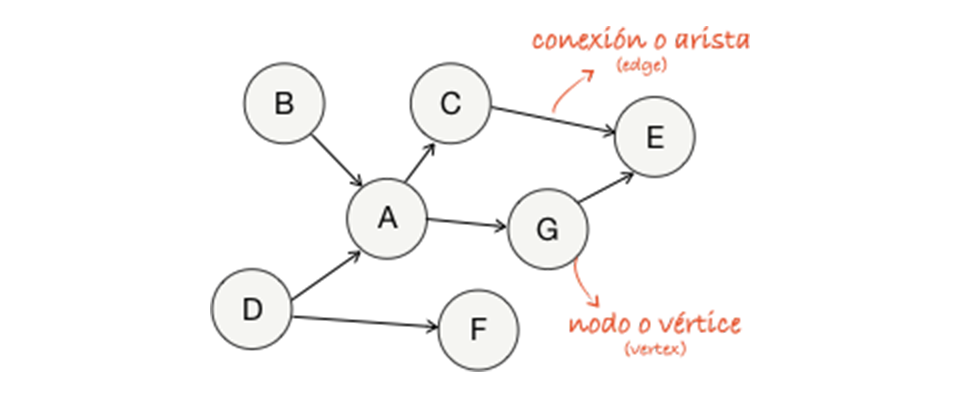
\includegraphics[width=.9\linewidth]{img/graph-example.png}  %%%%%%% POSIBLE CAMBIO POR DIBUJO DE GRAFO %%%%%%%%%%%%%%%



\tikzset{every picture/.style={line width=0.75pt}} %set default line width to 0.75pt        
\begin{center}
    
\begin{tikzpicture}[x=0.75pt,y=0.75pt,yscale=-1,xscale=1]
%uncomment if require: \path (0,235); %set diagram left start at 0, and has height of 235

%Shape: Ellipse [id:dp46037192501424906] 
\draw   (28,41.8) .. controls (28,31.95) and (36.74,23.97) .. (47.53,23.97) .. controls (58.31,23.97) and (67.05,31.95) .. (67.05,41.8) .. controls (67.05,51.64) and (58.31,59.62) .. (47.53,59.62) .. controls (36.74,59.62) and (28,51.64) .. (28,41.8) -- cycle ;
%Shape: Ellipse [id:dp8666875874865274] 
\draw   (28,132.35) .. controls (28,122.51) and (36.74,114.52) .. (47.53,114.52) .. controls (58.31,114.52) and (67.05,122.51) .. (67.05,132.35) .. controls (67.05,142.19) and (58.31,150.17) .. (47.53,150.17) .. controls (36.74,150.17) and (28,142.19) .. (28,132.35) -- cycle ;
%Shape: Ellipse [id:dp8980064731841073] 
\draw   (86.58,86) .. controls (86.58,76.16) and (95.32,68.18) .. (106.1,68.18) .. controls (116.89,68.18) and (125.63,76.16) .. (125.63,86) .. controls (125.63,95.85) and (116.89,103.83) .. (106.1,103.83) .. controls (95.32,103.83) and (86.58,95.85) .. (86.58,86) -- cycle ;
%Shape: Ellipse [id:dp34932880442543934] 
\draw   (137.35,36.81) .. controls (137.35,26.96) and (146.09,18.98) .. (156.87,18.98) .. controls (167.65,18.98) and (176.4,26.96) .. (176.4,36.81) .. controls (176.4,46.65) and (167.65,54.63) .. (156.87,54.63) .. controls (146.09,54.63) and (137.35,46.65) .. (137.35,36.81) -- cycle ;
%Shape: Ellipse [id:dp278308806793246] 
\draw   (187.33,103.83) .. controls (187.33,93.99) and (196.07,86) .. (206.86,86) .. controls (217.64,86) and (226.38,93.99) .. (226.38,103.83) .. controls (226.38,113.67) and (217.64,121.65) .. (206.86,121.65) .. controls (196.07,121.65) and (187.33,113.67) .. (187.33,103.83) -- cycle ;
%Shape: Ellipse [id:dp09615716654164908] 
\draw   (244.35,53.21) .. controls (244.35,43.36) and (253.09,35.38) .. (263.87,35.38) .. controls (274.66,35.38) and (283.4,43.36) .. (283.4,53.21) .. controls (283.4,63.05) and (274.66,71.03) .. (263.87,71.03) .. controls (253.09,71.03) and (244.35,63.05) .. (244.35,53.21) -- cycle ;
%Shape: Ellipse [id:dp2735336224480628] 
\draw   (131.88,150.17) .. controls (131.88,140.33) and (140.62,132.35) .. (151.4,132.35) .. controls (162.19,132.35) and (170.93,140.33) .. (170.93,150.17) .. controls (170.93,160.02) and (162.19,168) .. (151.4,168) .. controls (140.62,168) and (131.88,160.02) .. (131.88,150.17) -- cycle ;
%Straight Lines [id:da9533386093024172] 
\draw    (63.15,53.92) -- (88.83,71.33) ;
\draw [shift={(90.48,72.46)}, rotate = 214.14] [color={rgb, 255:red, 0; green, 0; blue, 0 }  ][line width=0.75]    (10.93,-3.29) .. controls (6.95,-1.4) and (3.31,-0.3) .. (0,0) .. controls (3.31,0.3) and (6.95,1.4) .. (10.93,3.29)   ;
%Straight Lines [id:da5146031298198329] 
\draw    (62.73,119.8) -- (91.18,99.98) ;
\draw [shift={(92.83,98.84)}, rotate = 145.14] [color={rgb, 255:red, 0; green, 0; blue, 0 }  ][line width=0.75]    (10.93,-3.29) .. controls (6.95,-1.4) and (3.31,-0.3) .. (0,0) .. controls (3.31,0.3) and (6.95,1.4) .. (10.93,3.29)   ;
%Straight Lines [id:da6897768644081719] 
\draw    (67.05,132.35) -- (129.95,149.64) ;
\draw [shift={(131.88,150.17)}, rotate = 195.37] [color={rgb, 255:red, 0; green, 0; blue, 0 }  ][line width=0.75]    (10.93,-3.29) .. controls (6.95,-1.4) and (3.31,-0.3) .. (0,0) .. controls (3.31,0.3) and (6.95,1.4) .. (10.93,3.29)   ;
%Straight Lines [id:da12271299201598895] 
\draw    (118.18,72.03) -- (140.98,49.2) ;
\draw [shift={(142.4,47.79)}, rotate = 134.96] [color={rgb, 255:red, 0; green, 0; blue, 0 }  ][line width=0.75]    (10.93,-3.29) .. controls (6.95,-1.4) and (3.31,-0.3) .. (0,0) .. controls (3.31,0.3) and (6.95,1.4) .. (10.93,3.29)   ;
%Straight Lines [id:da7174705901790854] 
\draw    (176.4,36.81) -- (242.4,52.74) ;
\draw [shift={(244.35,53.21)}, rotate = 193.57] [color={rgb, 255:red, 0; green, 0; blue, 0 }  ][line width=0.75]    (10.93,-3.29) .. controls (6.95,-1.4) and (3.31,-0.3) .. (0,0) .. controls (3.31,0.3) and (6.95,1.4) .. (10.93,3.29)   ;
%Straight Lines [id:da029993368368729123] 
\draw    (218.94,91.99) -- (251.67,68.9) ;
\draw [shift={(253.3,67.75)}, rotate = 144.8] [color={rgb, 255:red, 0; green, 0; blue, 0 }  ][line width=0.75]    (10.93,-3.29) .. controls (6.95,-1.4) and (3.31,-0.3) .. (0,0) .. controls (3.31,0.3) and (6.95,1.4) .. (10.93,3.29)   ;
%Straight Lines [id:da8448266168342549] 
\draw    (125.63,86) -- (185.41,103.27) ;
\draw [shift={(187.33,103.83)}, rotate = 196.11] [color={rgb, 255:red, 0; green, 0; blue, 0 }  ][line width=0.75]    (10.93,-3.29) .. controls (6.95,-1.4) and (3.31,-0.3) .. (0,0) .. controls (3.31,0.3) and (6.95,1.4) .. (10.93,3.29)   ;
%Straight Lines [id:da20461584691348] 
\draw [color={rgb, 255:red, 208; green, 2; blue, 27 }  ,draw opacity=1 ]   (208.11,15.7) -- (170.92,22.47) ;
\draw [shift={(168.95,22.83)}, rotate = 349.68] [color={rgb, 255:red, 208; green, 2; blue, 27 }  ,draw opacity=1 ][line width=0.75]    (10.93,-3.29) .. controls (6.95,-1.4) and (3.31,-0.3) .. (0,0) .. controls (3.31,0.3) and (6.95,1.4) .. (10.93,3.29)   ;
%Straight Lines [id:da668409998381462] 
\draw [color={rgb, 255:red, 208; green, 2; blue, 27 }  ,draw opacity=1 ]   (263.35,97.41) -- (237.8,80.96) ;
\draw [shift={(236.12,79.87)}, rotate = 32.79] [color={rgb, 255:red, 208; green, 2; blue, 27 }  ,draw opacity=1 ][line width=0.75]    (10.93,-3.29) .. controls (6.95,-1.4) and (3.31,-0.3) .. (0,0) .. controls (3.31,0.3) and (6.95,1.4) .. (10.93,3.29)   ;


% Text Node
\draw (42.42,34.51) node [anchor=north west][inner sep=0.75pt]   [align=left] {V};
% Text Node
\draw (42.42,125.06) node [anchor=north west][inner sep=0.75pt]   [align=left] {V};
% Text Node
\draw (100.99,78.72) node [anchor=north west][inner sep=0.75pt]   [align=left] {V};
% Text Node
\draw (151.76,29.52) node [anchor=north west][inner sep=0.75pt]   [align=left] {V};
% Text Node
\draw (201.75,96.54) node [anchor=north west][inner sep=0.75pt]   [align=left] {V};
% Text Node
\draw (258.76,45.92) node [anchor=north west][inner sep=0.75pt]   [align=left] {V};
% Text Node
\draw (146.29,142.89) node [anchor=north west][inner sep=0.75pt]   [align=left] {V};
% Text Node
\draw (202.38,8.13) node [anchor=north west][inner sep=0.75pt]   [align=left] {\textcolor[rgb]{0.82,0.01,0.11}{Vértice}};
% Text Node
\draw (257.93,89.41) node [anchor=north west][inner sep=0.75pt]   [align=left] {\textcolor[rgb]{0.82,0.01,0.11}{Arista}};


\end{tikzpicture}
\end{center}

El proyecto se centra en la implementación y exploración de estructuras de datos para grafos, por lo cual se hará uso particular del lenguaje de programación \textbf{C++} para la implementación y funcionamiento lógico, así como el uso de \textbf{Qt5}, un framework de desarrollo de software multiplataforma que permite crear aplicaciones gráficas para múltiples sistemas operativos. Con ayuda de estas herramientas se plantea la elaboración de una aplicación que permite a los usuarios explorar de manera gráfica las operaciones aplicables a la estructura de un grafo. Cabe destacar que la elaboración de este proyecto se fundamenta en el Capítulo 12 \"{}Graphs\"{} del libro \"{}Open Data Structures\"{}.\cite{ODS} \\
Este capítulo es un componente esencial para entender la aplicación de grafos en su forma de Matrices de Adyacencia y Listas de Adyacencia, así como sus técnicas de recorrido, como la búsqueda en Amplitud y la búsqueda en Profundidad.\\

Dentro de este reporte abordarán los conceptos teóricos presentados en el libro a través de la implementación y análisis de algoritmos relacionados con la Representación y el Recorrido de Grafos.

 
\section{Desarrollo Experimental}

C++ ha evolucionado a partir del lenguaje de programación C, y con el tiempo, ha experimentado una mayor evolución y desarrollo desde su definición original. Ha permitido la introducción de características que no formaban parte de C, como constantes simbólicas, sustitución de funciones en línea, tipos de referencia, polimorfismo paramétrico a través de plantillas y excepciones (que se discuten más adelante). Como resultado, C++ ha crecido hasta convertirse en un lenguaje de programación complejo y seguro.\cite{C++} \\
Los sistemas lógicos de grafos en C++ se beneficia de estas mejoras, permitiendo una manipulación eficiente de los datos y una mayor flexibilidad en la implementación de algoritmos. De este modo, hace posible la manipulación de punteros y referencias, así como la creación de estructuras de datos complejas entre los cuales se pueden destacar las listas enlazadas, matrices de adyacencia y listas de adyacencia; de esta forma facilitando la representación y manipulación de grafos.\\
La implementación de C++ se centró en la creación de una estructura de datos robusta y eficiente para grafos. Se consideraron varias estructuras, como listas enlazadas, matrices de adyacencia y listas de adyacencia, y se eligieron basándose en los requisitos específicos del proyecto y en su eficiencia en diferentes contextos.\\

Después de explorar los fundamentos de los grafos y su implementación en C++, es importante destacar la importancia de Qt como un framework que facilita el desarrollo de aplicaciones gráficas y lógicas de grafos de manera eficiente y multiplataforma. Qt5 ha evolucionado desde una sencilla biblioteca de clases hasta un amplio framework, el cual ha mejorado la calidad de su entorno de desarrollo, \textit{Qt Creator}, y su compatibilidad con más lenguajes y plataformas gracias a su línea de comandos (CLI). Así, el equipo de Qt ha conferido siempre una gran importancia a abarcar también campos de aplicación específicos de los sectores de la computación de escritorio, así como de los dispositivos móviles, ofreciendo una amplia gama de bibliotecas y módulos de desarrollo.\cite{Qt}\\
Su integración se llevó a cabo para desarrollar una interfaz gráfica de usuario (GUI) que permita a los usuarios interactuar con las estructuras de datos de grafos de manera intuitiva. Además de su capacidad para desarrollar aplicaciones gráficas multiplataforma y por su amplia gama de herramientas y widgets, destacando los elementos de Creación de Ventanas, Entrada de Dato y Visualización de Resultados.

\begin{center}
    \textit{En el contexto de este proyecto, los grafos juegan un papel central.}\\%%%%%%%%%%%%%%%%%%%%%%%%%%
\end{center}

Existen dos formas estándar de representar un grafo: como una colección de \textit{\textbf{listas de adyacencia}} (Partiendo de los nodos de cada vértice, evoluciona una lista que informa los nodos que son adyacentes del inicial) o como una \textit{\textbf{matriz de adyacencia}} ( matrices cuadradas de tantas filas y columnas como vértices tenga el grafo a representar. En las celdas de la matriz se indica si existe un arco entre los vértices que determinan la celda). Cualquiera de las dos formas se aplica tanto a los grafos dirigidos como a los no dirigidos. \cite{Adyacencias}

Asimismo, algunas operaciones básicas realizadas en grafos son: addEdge, removeEdge, hasEdge, outEdges, inEdges que son esenciales para su manipulación. Estas operaciones permiten a los desarrolladores interactuar con la estructura de datos del grafo, modificándola según sea necesario para el proyecto.\cite{FuncionesGraphs}

Además de algoritmos de búsqueda en grafos, como la búsqueda en amplitud (Breadth-First Search, BFS) llamada así porque expande la frontera entre vértices descubiertos y no descubiertos uniformemente a lo ancho de la frontera; y la búsqueda en profundidad (Depth-First Search, DFS) que como su nombre indica, busca \textit{más profundo} en el grafo siempre que sea posible. La búsqueda en profundidad explora los bordes que salen del vértice más recién descubierto v que aún tiene bordes no explorados que salen de él.\cite{BFS&DFS}\\
Estos algoritmos son fundamentales para explorar y analizar la estructura de los grafos.\\
Para validar procesos y asegurar la correcta funcionalidad de las Implementaciones en C++ y las Interfaces en Qt5, se llevaron a cabo pruebas de integración, pruebas de usabilidad, y pruebas de rendimiento para verificar la eficiencia de las operaciones realizadas en distintos sistemas.\\
Las pruebas revelaron que la aplicación funciona como se esperaba, permitiendo a los usuarios interactuar con grafos de manera efectiva y visualizar los resultados de las operaciones realizadas. \textbf{Los resultados obtenidos confirman la eficacia de la implementación en C++ y la eficaz integración con Qt5}



\section{Resultados}

El desarrollo del proyecto resultó en una aplicación gráfica interactiva que permite a los usuarios manipular y explorar estructuras de datos para grafos de manera visual. Esta aplicación, construida con C++ y Qt5, proporciona una plataforma robusta para la creación, visualización y análisis de grafos. A continuación, se detallan los resultados obtenidos en cada una de las funcionalidades implementadas así como si respectiva captura de pantalla.

%\begin{center}
%    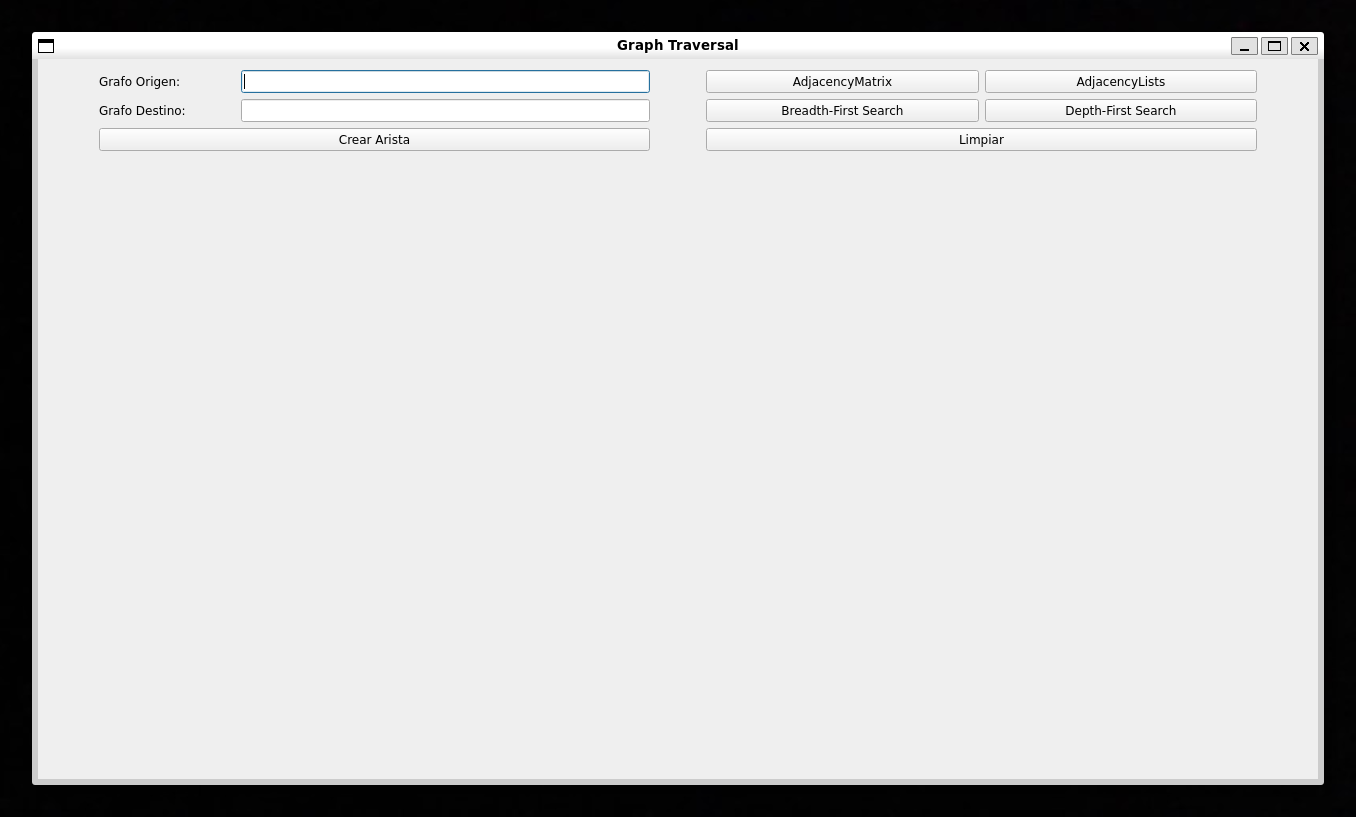
\includegraphics[width=\linewidth]{img/inicio.png}
%    \captionof{figure}{Pantalla de Inicio}
%\end{center}



\subsubsection{\textbf{Creación de Vértices}}
El componente principal del sistema es el área de dibujo, donde los usuarios pueden interactuar para crear grafos. La aplicación permite dibujar vértices al hacer clic dentro del área . Esta funcionalidad es esencial para la construcción de grafos, ya que cada clic representa la adición de un nuevo vértice al grafo. Los vértices se pueden agregar libremente, lo que permitirá a los usuarios diseñar grafos complejos y personalizados.
\begin{center}
    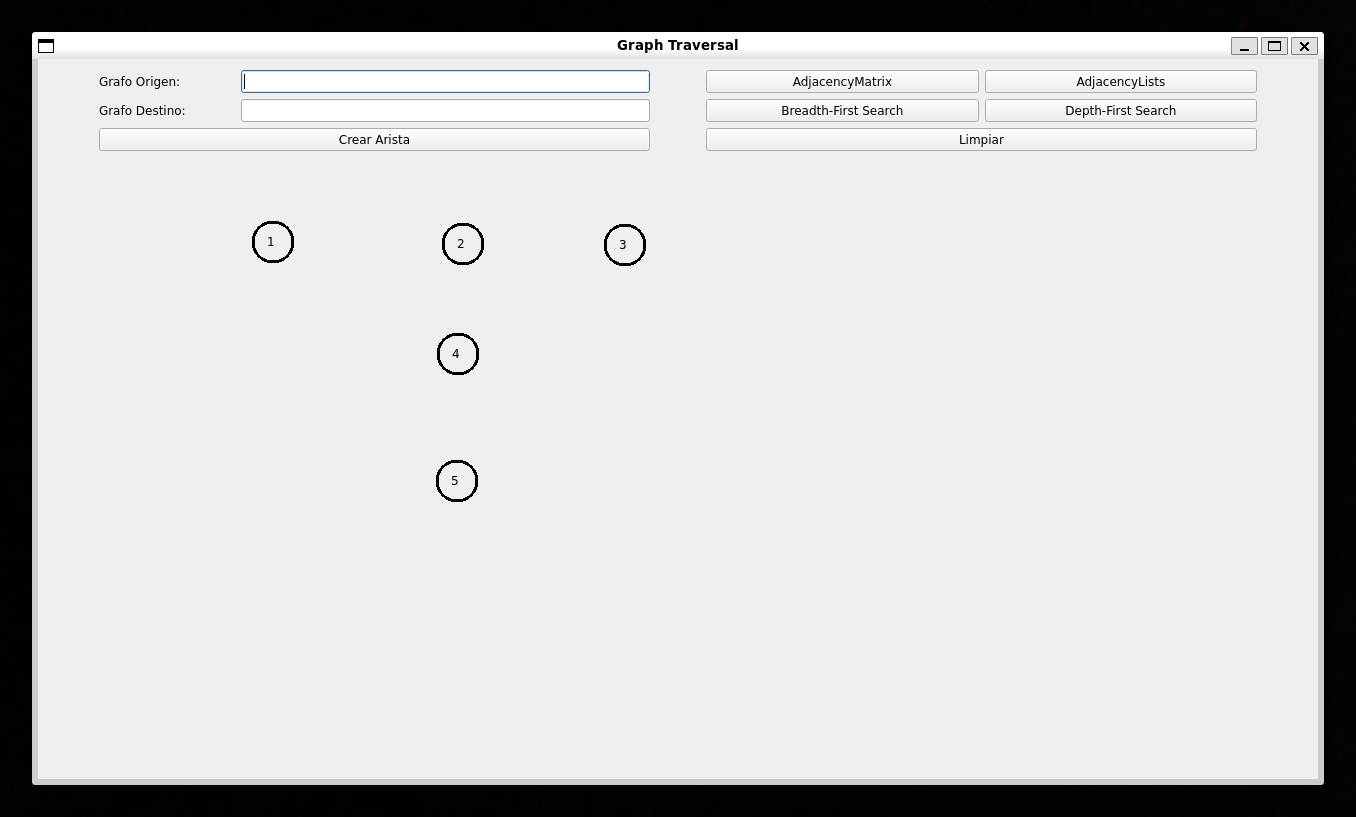
\includegraphics[width=\linewidth]{img/Vertices.png}
    \captionof{figure}{Adición de Vértices}
\end{center}



\subsubsection{\textbf{Dibujo de Aristas}}
Para complementar el sistema de dibujo, se implementó una funcionalidad en la cual se le solicita al usuario ingresar los números de los vértice de origen y de destino para dibujar una arista que los una. Esta característica es crucial para definir las conexiones entre los vértices, permitiendo así la representación de relaciones o procesos entre objetos en el grafo.
\begin{center}
    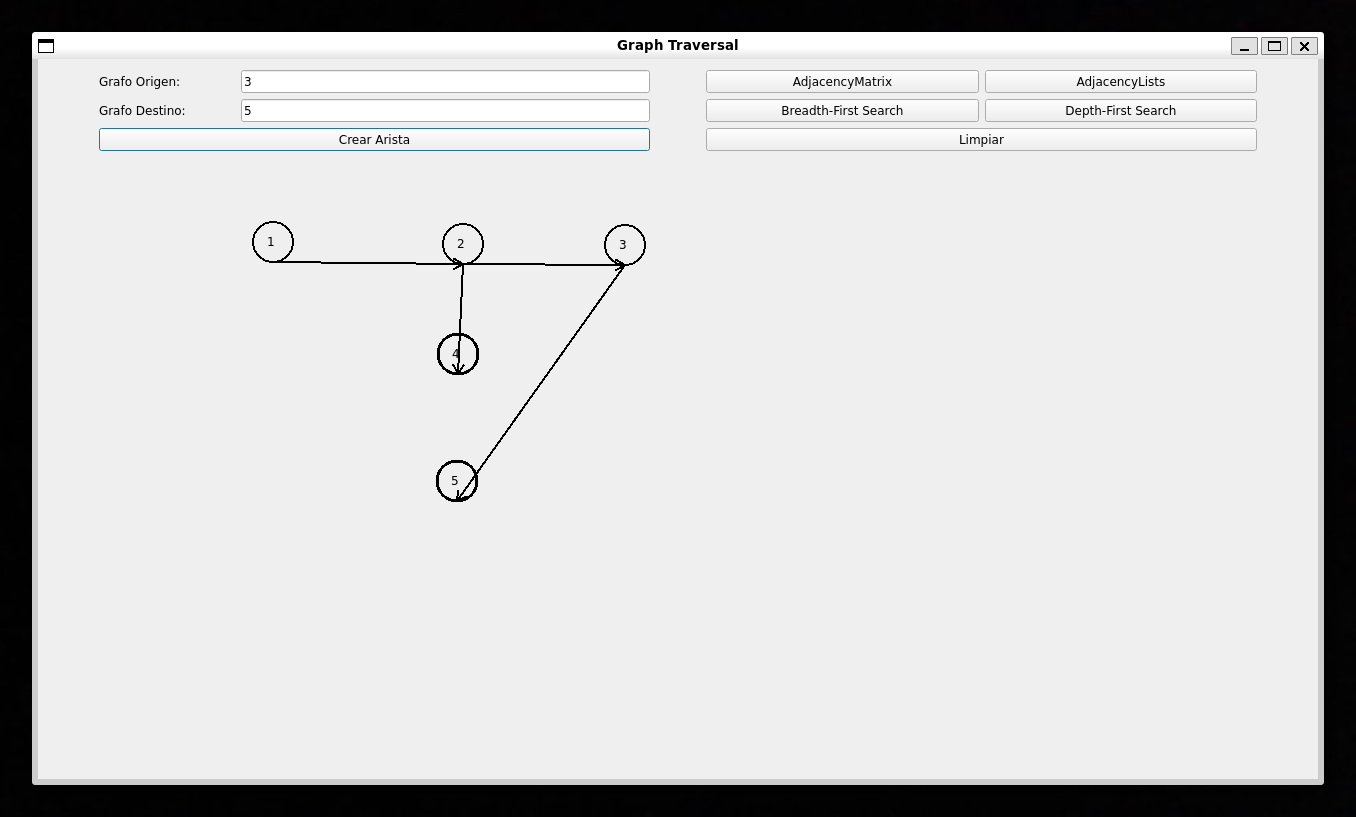
\includegraphics[width=\linewidth]{img/Aristas.png}
    \captionof{figure}{Trazado de Aristas}
\end{center}



\subsubsection{\textbf{Generación de Matrices y Listas de Adyacencia}}
La aplicación cuenta con botones para generar tanto una matriz de adyacencia como una lista de adyacencia del grafo actualmente dibujado. Estas representaciones permiten una comprensión más profunda de la estructura del grafo, facilitando el análisis de sus propiedades y la aplicación de algoritmos específicos.\\
\begin{itemize}
    \item \textbf{Matriz de Adyacencia}: Representa las conexiones entre los vértices del grafo mediante una matriz cuadrada. Cada entrada en la matriz indica la presencia (1) o ausencia (0) de una arista entre dos vértices.
        \begin{center}
            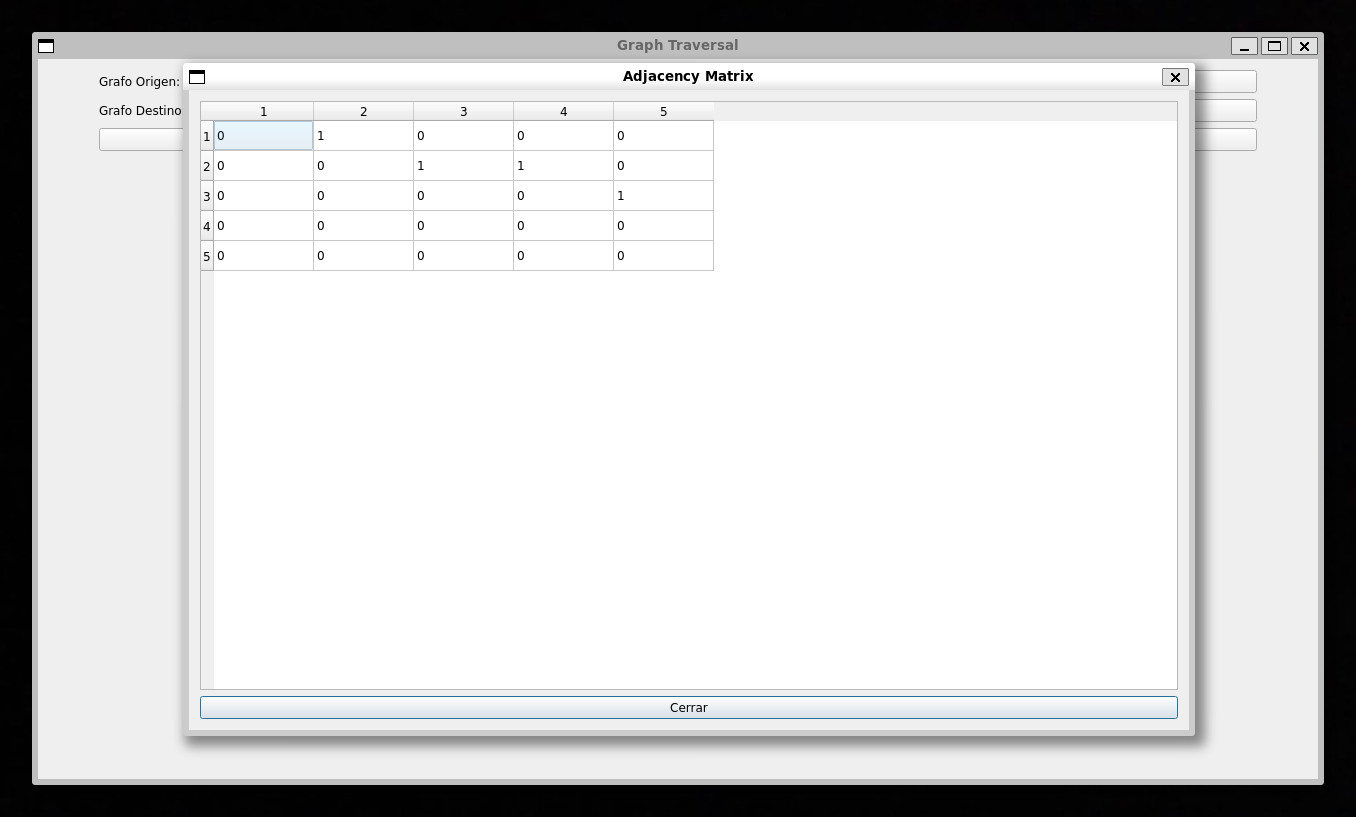
\includegraphics[width=\linewidth]{img/AdjencyMatrix.png}
            \captionof{figure}{Matriz de Adyacencia}
        \end{center}
    \item \textbf{Lista de Adyacencia}: Ofrece una representación alternativa donde cada vértice tiene una lista de sus vértices adyacentes. Esta representación es más eficiente en términos de espacio para grafos dispersos.
        \begin{center}
            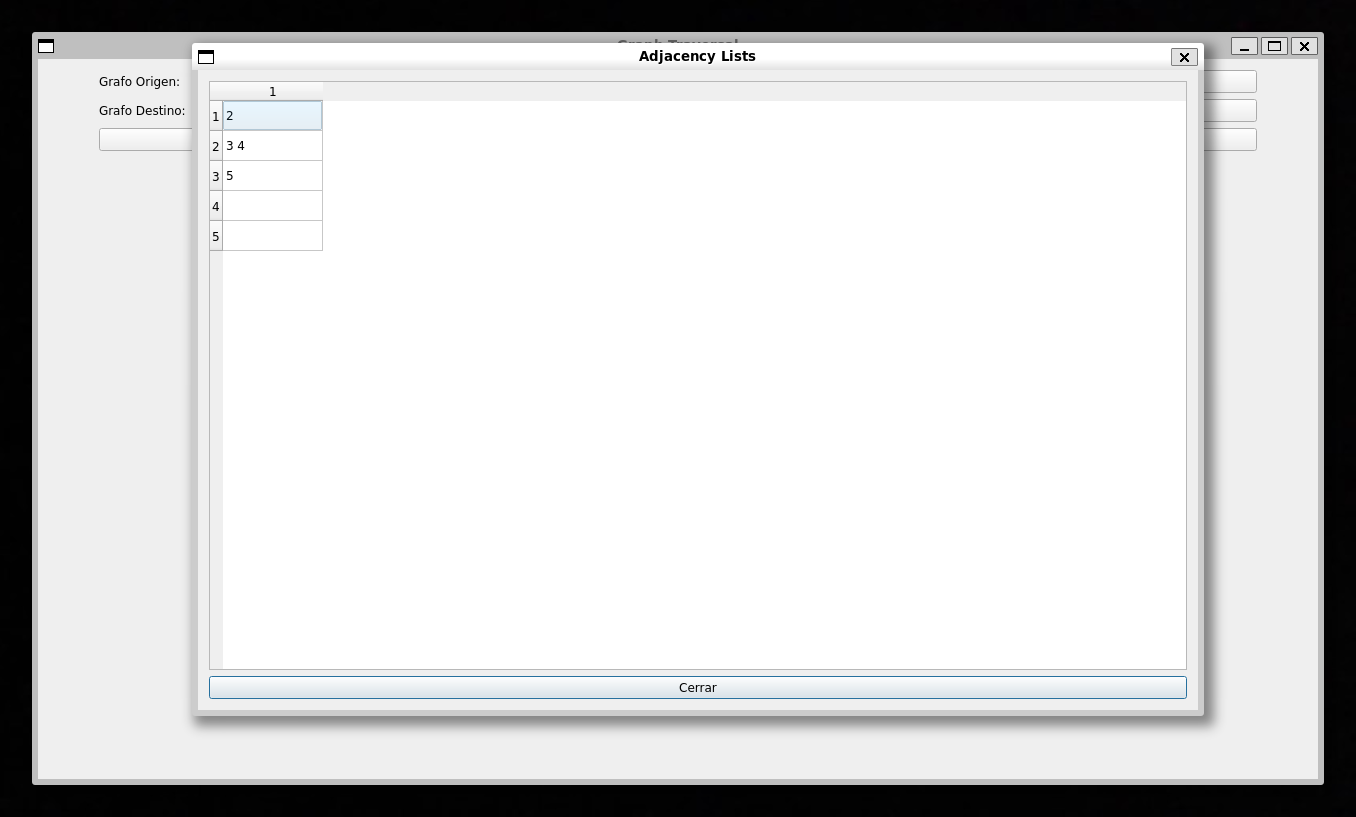
\includegraphics[width=\linewidth]{img/AdjencyLists.png}
            \captionof{figure}{Lista de Adyacencia}
        \end{center}
\end{itemize}



\subsubsection{\textbf{Algoritmos de Búsqueda}}
La aplicación incluye botones para realizar búsquedas en profundidad y búsqueda en amplitud en el grafo. Estos algoritmos son fundamentales para explorar y analizar la estructura de los grafos, permitiendo encontrar caminos entre vértices, identificar componentes conectados, y más.
\begin{itemize}
    \item \textbf{Búsqueda en Amplitud (BFS)}: En esta se comienza en un vértice raíz y se comienza a explorar los vértices vecinos a corta distancia antes de pasar a los vértices más lejanos. Es particularmente útil para encontrar el camino más corto entre dos vértices en un grafo no ponderado.\\
    Para su ejecución se activa el botón, el cual manda a llamar la función de búsqueda en amplitud para que esta realice el recorrido de los vértices, registre su alcance e imprima la información en una ventana nueva ventana.
        \begin{center}
            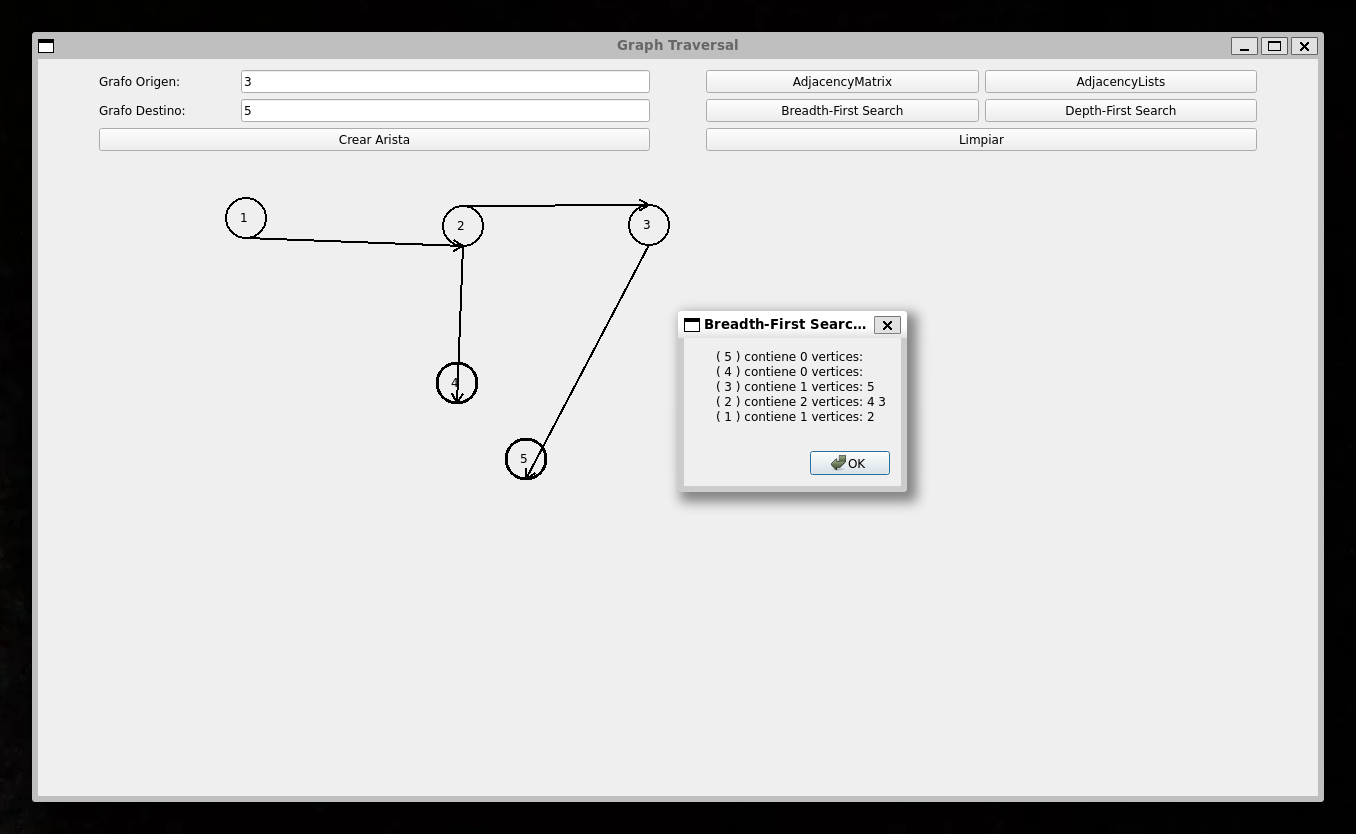
\includegraphics[width=\linewidth]{img/BFS.png}
            \captionof{figure}{Breadth-First Search}
        \end{center}
    \item \textbf{Búsqueda en Profundidad (DFS)}: Se comienza en un vértice raíz y se busca explorar tan lejos como sea posible, a lo largo de cada rama antes de retroceder. Es útil para identificar todos los caminos posibles entre dos vértices o para encontrar componentes conectados.\\
    Su botón manda llamar a la función de búsqueda en profundidad, la cual explorara los vértices, registrara aquellos vértices contenidos en el recorrido e imprime los resultados en una nueva ventana.
        \begin{center}
            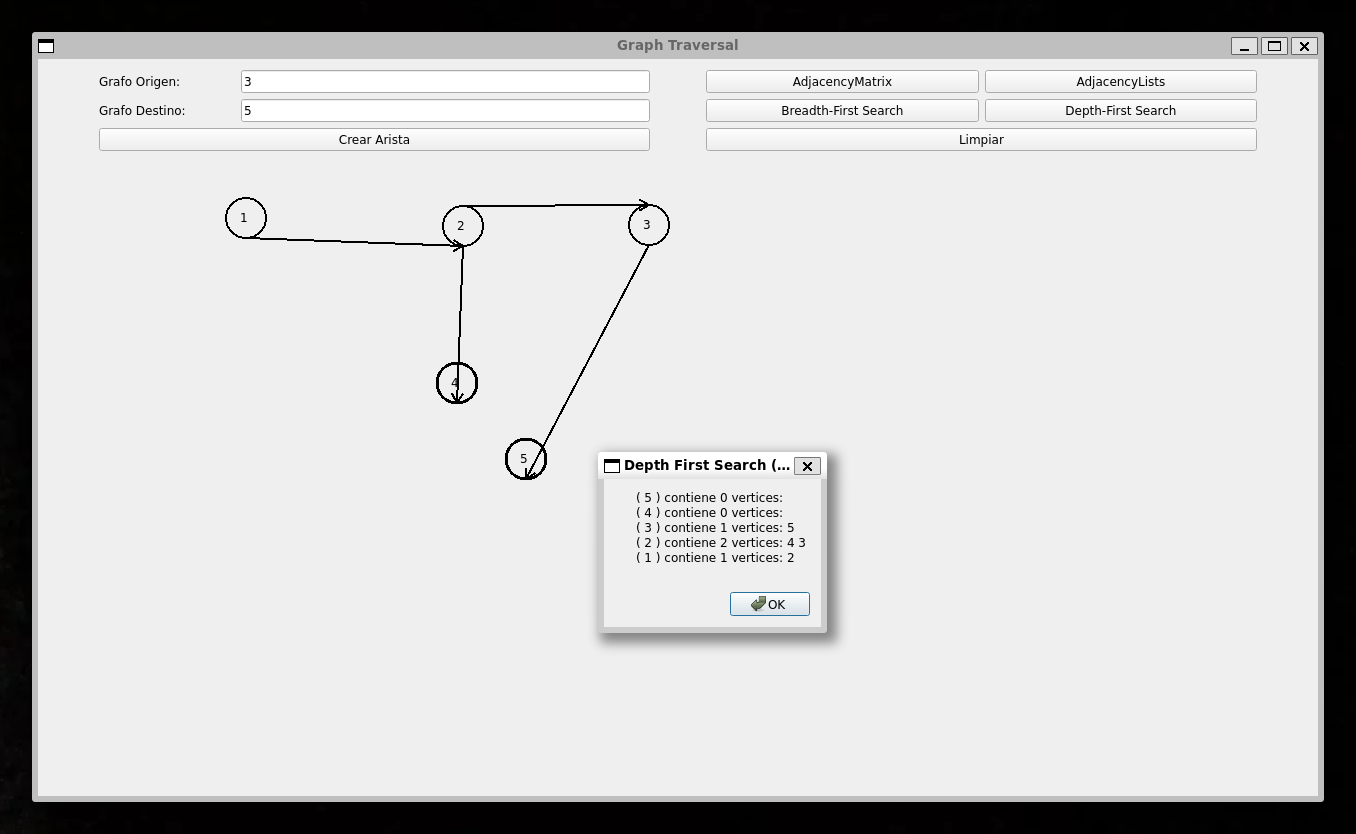
\includegraphics[width=\linewidth]{img/DFS.png}
            \captionof{figure}{Deep-First Search}
        \end{center}
\end{itemize}

En resumen, los resultados obtenidos demuestran la eficacia de la aplicación en la creación, visualización y análisis de grafos. La implementación de estas funcionalidades en C++ y Qt5 ha permitido desarrollar una herramienta interactiva y visualmente intuitiva que facilita la comprensión de las estructuras de datos para grafos y sus aplicaciones. La cual se encuentra publicada en github. \cite{GitHub2024}



\section{Conclusión}

En este proyecto, se abordó la implementación y exploración de estructuras de datos para grafos mediante el lenguaje de programación C++ y el framework Qt5, basándonos en el libro \"{}Open Data Structures\"{}. Se buscó responder a los desafíos de representar y manipular grafos de manera eficiente y visualmente interactiva. A través de la implementación de listas de adyacencia y la integración de interfaces gráficas en Qt5, se logró una comprensión profunda de cómo las estructuras de datos pueden modelar y resolver problemas complejos, facilitando la visualización y análisis de grafos.

Los resultados obtenidos demostraron la eficacia de las estructuras de datos para grafos y la importancia de las interfaces gráficas para facilitar la interacción con estas estructuras. La aplicación de algoritmos de búsqueda en grafos, como la búsqueda en amplitud y la búsqueda en profundidad, permitió explorar y analizar la estructura de los grafos de manera intuitiva. La implementación exitosa de estas técnicas proporcionó una plataforma sólida para la exploración y comprensión de los conceptos de grafos y algoritmos.

Este proyecto no solo fortaleció nuestras habilidades en programación y desarrollo de software, sino que también enriqueció nuestro entendimiento de cómo las estructuras de datos y los algoritmos pueden aplicarse en situaciones prácticas. Los conocimientos adquiridos en este proyecto son fundamentales para futuros proyectos que involucren modelado de problemas complejos y desarrollo de aplicaciones interactivas. La integración de teoría y práctica, a través de la implementación en C++ y la interfaz gráfica en Qt5, demostró ser una estrategia efectiva para abordar los desafíos de la programación y el análisis de datos.



\printbibliography



\end{document}
